% PrivacyGNN beginner-first full guide
% Build:
%   cd privacy-gnn/docs
%   pdflatex PROJECT_BEGINNER_FULL_GUIDE.tex
%   pdflatex PROJECT_BEGINNER_FULL_GUIDE.tex
\documentclass[11pt,a4paper]{article}
\usepackage[margin=0.82in]{geometry}
\usepackage[T1]{fontenc}
\usepackage{lmodern}
\usepackage{microtype}
\usepackage{xcolor}
\usepackage{hyperref}
\usepackage{booktabs}
\usepackage{array}
\usepackage{longtable}
\usepackage{amsmath}
\usepackage{tikz}
\usetikzlibrary{arrows.meta,positioning,calc,shapes.geometric}

\hypersetup{
  colorlinks=true,
  linkcolor=blue!55!black,
  urlcolor=blue!55!black,
  citecolor=blue!55!black
}

\definecolor{deep}{HTML}{0F172A}
\definecolor{textgray}{HTML}{334155}
\definecolor{softblue}{HTML}{EFF6FF}
\definecolor{softgreen}{HTML}{ECFDF5}
\definecolor{softorange}{HTML}{FFF7ED}
\definecolor{softred}{HTML}{FEF2F2}
\definecolor{softpurple}{HTML}{F5F3FF}
\definecolor{softgray}{HTML}{F8FAFC}
\definecolor{accent}{HTML}{0F766E}

\setlength{\parindent}{0pt}
\setlength{\parskip}{0.65em}
\renewcommand{\arraystretch}{1.24}
\newcolumntype{L}[1]{>{\raggedright\arraybackslash}p{#1}}

\makeatletter
\def\@listi{\leftmargin\leftmargini \topsep 4pt \parsep 2pt \itemsep 2pt}
\makeatother

\newcommand{\code}[1]{\texttt{\detokenize{#1}}}
\newcommand{\important}[1]{\textbf{\textcolor{accent}{#1}}}

\title{\textbf{PrivacyGNN Beginner Full Guide}\\
\large A slow, plain-English explanation of the entire project}
\author{Prepared for Krish Sharma}
\date{\today}

\begin{document}
\maketitle

\begin{abstract}
This guide explains the PrivacyGNN project from the ground up. It assumes you are new to machine learning privacy, graph neural networks, experiment code, and research result files. The goal is not just to say what each file does, but to explain why it exists, what problem it solves, how the pieces connect, and what you should think while reading the code. It intentionally repeats ideas in different ways because beginners learn best when the same idea is seen from multiple angles.
\end{abstract}

\tableofcontents
\newpage

%==============================================================================
\section{How to Use This Guide}
%==============================================================================

This is a beginner-first guide. That means it moves slowly. If something feels obvious, you can skim it. If something feels confusing, pause and reread the example. The goal is that by the end you can explain your project to another person without just memorizing file names.

There are three levels of understanding:

\begin{enumerate}
  \item \textbf{Story level:} What question is the project trying to answer?
  \item \textbf{Experiment level:} What is actually run, measured, saved, and plotted?
  \item \textbf{Code level:} Which file/function performs each step?
\end{enumerate}

Most confusion happens when these levels get mixed together. For example, ``membership inference attack'' is a research idea, but \code{confidence_attack} in \code{attacks.py} is the actual code implementation of one attack. This guide keeps those apart.

\textbf{Recommended reading plan:}
\begin{itemize}
  \item First pass: read Sections 1--8 to understand the big ideas.
  \item Second pass: read Sections 9--18 with the code open beside you.
  \item Third pass: use Sections 19--25 as your reference when running experiments or explaining results.
\end{itemize}

%==============================================================================
\section{The Project in One Sentence}
%==============================================================================

\textbf{PrivacyGNN studies whether graph neural networks reveal which nodes were used during training, and whether simple defenses can reduce that leakage without hurting accuracy too much.}

That sentence has many parts:

\begin{itemize}
  \item \textbf{Graph neural networks:} machine learning models that learn from points connected by edges.
  \item \textbf{Reveal which nodes were used during training:} privacy leakage called membership inference.
  \item \textbf{Simple defenses:} practical tricks like dropping edges, smoothing labels, masking confidence scores, or stopping early.
  \item \textbf{Without hurting accuracy:} the privacy-utility tradeoff.
\end{itemize}

The project is not just one model. It is a whole experiment system:

\begin{center}
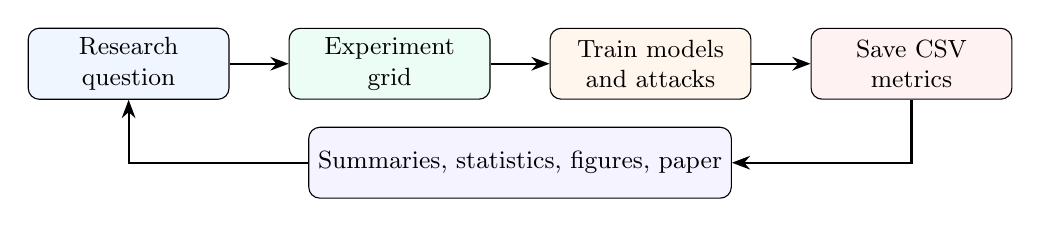
\begin{tikzpicture}[
  font=\small,
  box/.style={draw,rounded corners,align=center,minimum width=2.55cm,minimum height=0.9cm},
  arr/.style={-{Stealth},thick}
]
\node[box,fill=softblue] (q) {Research\\question};
\node[box,fill=softgreen,right=0.75cm of q] (grid) {Experiment\\grid};
\node[box,fill=softorange,right=0.75cm of grid] (run) {Train models\\and attacks};
\node[box,fill=softred,right=0.75cm of run] (results) {Save CSV\\metrics};
\node[box,fill=softpurple,below=0.8cm of $(grid)!0.5!(run)$] (fig) {Summaries, statistics, figures, paper};
\draw[arr] (q) -- (grid);
\draw[arr] (grid) -- (run);
\draw[arr] (run) -- (results);
\draw[arr] (results) |- (fig.east);
\draw[arr] (fig.west) -| (q.south);
\end{tikzpicture}
\end{center}

%==============================================================================
\section{A Beginner Analogy}
%==============================================================================

Imagine a teacher trains for an exam using a private study list of students. Later, someone asks the teacher questions about many students and watches how confident the teacher sounds.

If the teacher sounds extremely confident about certain students and less confident about others, an attacker may guess: ``The very confident ones were probably on the private study list.''

That is the core idea of a membership inference attack.

Now replace the teacher with a machine learning model:

\begin{itemize}
  \item The \textbf{private study list} is the training set.
  \item The \textbf{students} are graph nodes.
  \item The \textbf{teacher's confidence} is the model's predicted probability.
  \item The \textbf{attacker's guess} is member vs non-member.
\end{itemize}

The project asks: does this guessing work better for graph neural networks? And can we make it harder?

%==============================================================================
\section{What Is a Graph?}
%==============================================================================

A graph is a set of objects and relationships.

\begin{itemize}
  \item Objects are called \textbf{nodes}.
  \item Relationships are called \textbf{edges}.
\end{itemize}

Examples:
\begin{itemize}
  \item In a social network, people are nodes and friendships are edges.
  \item In a citation network, papers are nodes and citations are edges.
  \item In a medical graph, patients or conditions can be nodes and relationships can be edges.
\end{itemize}

In code, a graph is usually represented by:

\begin{itemize}
  \item \code{x}: node features, meaning numbers that describe each node.
  \item \code{edge_index}: pairs of node IDs that say which nodes are connected.
  \item \code{y}: labels, meaning the correct class for each node.
  \item \code{train_mask}: which nodes are used for training.
  \item \code{test_mask}: which nodes are held out for testing.
\end{itemize}

In PyTorch Geometric, these live in a \code{Data} object.

\subsection{Tiny Example}

Suppose there are four papers:

\begin{itemize}
  \item Paper 0: Machine Learning
  \item Paper 1: Machine Learning
  \item Paper 2: Biology
  \item Paper 3: Biology
\end{itemize}

If Paper 0 cites Paper 1, and Paper 2 cites Paper 3, then the graph has edges:
\[
(0,1), (1,0), (2,3), (3,2)
\]
The project uses undirected-style edges by adding both directions.

%==============================================================================
\section{What Is Node Classification?}
%==============================================================================

Node classification means predicting the label of a node.

In this project, every node has a label like:

\[
y_i \in \{0, 1, 2, 3, 4\}
\]

The model receives:
\begin{itemize}
  \item the node's feature vector,
  \item possibly the graph connections,
  \item labels for training nodes only.
\end{itemize}

The model outputs probabilities:

\[
\left[0.05,\ 0.10,\ 0.75,\ 0.04,\ 0.06\right]
\]

This means the model thinks class 2 is most likely.

\textbf{Accuracy} asks: did the model pick the correct class?

\textbf{Privacy attack AUC} asks: can an attacker use these probabilities to guess whether this node was in training?

Those are different questions.

%==============================================================================
\section{What Is Machine Learning Privacy Leakage?}
%==============================================================================

Many people think privacy is safe if the raw data is hidden. But machine learning models can leak information through their outputs.

Example:
\begin{itemize}
  \item The model never shows its training set.
  \item The model only shows prediction probabilities.
  \item But those probabilities may be unusually confident for training examples.
  \item An attacker can exploit this pattern.
\end{itemize}

This is why membership inference matters.

\subsection{Member and Non-Member}

In this project:

\begin{itemize}
  \item \textbf{Member} means the node was in the model's training set.
  \item \textbf{Non-member} means the node was not in training, usually in the test set.
\end{itemize}

The attacker tries to classify:

\[
\text{node} \rightarrow \text{member or non-member}
\]

\subsection{Why Confidence Matters}

Models often behave differently on examples they trained on:
\begin{itemize}
  \item They may be more confident.
  \item They may have lower entropy.
  \item They may put more probability on the true class.
\end{itemize}

These differences are exactly what the attacks in \code{attacks.py} measure.

%==============================================================================
\section{What Is a Graph Neural Network?}
%==============================================================================

A normal model like logistic regression or an MLP looks at one node's features by itself.

A graph neural network also looks at neighbors.

The simple idea:

\begin{quote}
To understand a node, look at the node and the nodes connected to it.
\end{quote}

\begin{center}
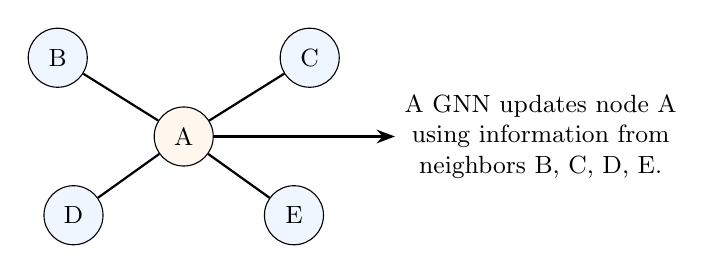
\begin{tikzpicture}[
  font=\small,
  node/.style={circle,draw,minimum size=0.75cm},
  arr/.style={-{Stealth},thick}
]
\node[node,fill=softorange] (c) at (0,0) {A};
\node[node,fill=softblue] (n1) at (-1.6,1) {B};
\node[node,fill=softblue] (n2) at (1.6,1) {C};
\node[node,fill=softblue] (n3) at (-1.4,-1) {D};
\node[node,fill=softblue] (n4) at (1.4,-1) {E};
\draw[thick] (c) -- (n1);
\draw[thick] (c) -- (n2);
\draw[thick] (c) -- (n3);
\draw[thick] (c) -- (n4);
\node[align=center,right=2.3cm of c] (txt) {A GNN updates node A\\using information from\\neighbors B, C, D, E.};
\draw[arr] (c) -- (txt);
\end{tikzpicture}
\end{center}

\subsection{Why This Could Affect Privacy}

Graph learning can affect privacy in two opposite ways:

\begin{itemize}
  \item It might \textbf{increase leakage} because a node's training information can spread through edges.
  \item It might \textbf{reduce leakage} because neighbor averaging can smooth predictions and reduce memorization.
\end{itemize}

Your project studies which actually happens under different graph structures.

%==============================================================================
\section{The Four Research Questions}
%==============================================================================

The README gives four research questions. Here they are in beginner language.

\subsection{RQ1: Are GNNs More Vulnerable Than Non-Graph Models?}

This compares:
\begin{itemize}
  \item LogReg and MLP: models that ignore edges.
  \item GCN and GraphSAGE: models that use edges.
\end{itemize}

The question is whether using graph structure makes membership attacks easier.

\subsection{RQ2: How Do Homophily and Density Affect Leakage?}

\textbf{Homophily} means similar nodes connect to each other.

\textbf{Density} means how many edges the graph has.

The project creates synthetic graphs where these can be changed separately:

\[
\text{high/low homophily} \times \text{sparse/medium/dense density}
\]

\subsection{RQ3: Can Lightweight Defenses Reduce Leakage?}

A defense is a change meant to make membership inference harder. The project tests simple defenses that are easy to run.

\subsection{RQ4: What Is the Utility-Privacy Tradeoff?}

Utility means the model is useful, usually high accuracy.

Privacy means the attack does poorly, usually attack AUC near 0.5.

The best situation is:
\[
\text{high accuracy} \quad \text{and} \quad \text{attack AUC near } 0.5.
\]

%==============================================================================
\section{The Whole Project Workflow}
%==============================================================================

The full project workflow looks like this:

\begin{center}
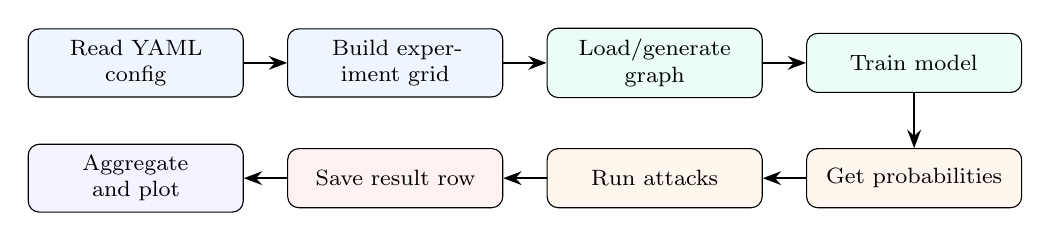
\begin{tikzpicture}[
  font=\footnotesize,
  box/.style={draw,rounded corners,align=center,text width=2.45cm,minimum height=0.75cm,inner sep=4pt},
  arr/.style={-{Stealth},thick}
]
\node[box,fill=softblue] (cfg) {Read YAML config};
\node[box,fill=softblue,right=0.55cm of cfg] (grid) {Build experiment grid};
\node[box,fill=softgreen,right=0.55cm of grid] (data) {Load/generate graph};
\node[box,fill=softgreen,right=0.55cm of data] (train) {Train model};
\node[box,fill=softorange,below=0.7cm of train] (predict) {Get probabilities};
\node[box,fill=softorange,left=0.55cm of predict] (attack) {Run attacks};
\node[box,fill=softred,left=0.55cm of attack] (save) {Save result row};
\node[box,fill=softpurple,left=0.55cm of save] (summary) {Aggregate and plot};
\draw[arr] (cfg) -- (grid);
\draw[arr] (grid) -- (data);
\draw[arr] (data) -- (train);
\draw[arr] (train) -- (predict);
\draw[arr] (predict) -- (attack);
\draw[arr] (attack) -- (save);
\draw[arr] (save) -- (summary);
\end{tikzpicture}
\end{center}

Each row in \code{results/all_results.csv} comes from one pass through this workflow.

%==============================================================================
\section{The Repository Map in Plain English}
%==============================================================================

\begin{longtable}{@{}L{0.28\textwidth}L{0.64\textwidth}@{}}
\toprule
\textbf{File} & \textbf{Beginner explanation}\\
\midrule
\endhead
\code{config.py} & Decides what experiments exist. It reads the YAML file and expands it into many combinations.\\
\code{experiment_config.yaml} & The main menu of experiment options: datasets, models, defenses, seeds, attacks.\\
\code{experiment_config_paper.yaml} & A smaller, cleaner menu for the paper-style experiment grid.\\
\code{data.py} & Creates or loads graph data. Also measures homophily and density.\\
\code{models.py} & Defines the two GNN model classes: GCN and GraphSAGE.\\
\code{training.py} & Teaches a GNN to classify nodes. Includes defense options.\\
\code{attacks.py} & Tries to guess train membership from model probabilities.\\
\code{experiment.py} & Runs one complete experiment: data, model, defense, attack, metrics.\\
\code{run_final.py} & Runs all experiments in the grid and writes CSV files.\\
\code{stats_utils.py} & Compares defenses statistically and computes bootstrap confidence intervals.\\
\code{generate_figures.py} & Makes paper-style figures from saved results.\\
\code{generate_basic_figures.py} & Makes simpler figures for understanding synthetic results.\\
\code{generate_final_visuals.py} & Makes polished final visuals for presentation/poster use.\\
\code{generate_poster_visuals.py} & Makes a larger poster visual suite.\\
\code{ogb_loader.py} & Placeholder for large graph datasets. Not active in this checkout.\\
\code{graph_minibatch.py} & Placeholder for minibatch training and DP-SGD. Not active in this checkout.\\
\code{lira_attack.py} & Placeholder for LiRA attack. Currently returns random-guess values.\\
\code{results/*.csv} & The actual experiment outputs. These are the source of truth.\\
\code{paper/} & Paper, manuscript, slide, and literature assets.\\
\bottomrule
\end{longtable}

%==============================================================================
\section{Configuration: The Experiment Menu}
%==============================================================================

The project is config-driven. This means you do not hard-code every experiment in Python. Instead, you write choices in YAML.

Think of \code{experiment_config_paper.yaml} like a restaurant menu:

\begin{itemize}
  \item datasets,
  \item models,
  \item attacks,
  \item defenses,
  \item training settings,
  \item seeds.
\end{itemize}

Then \code{config.py} combines them.

\subsection{What Is a Seed?}

A seed is a number that controls randomness. If you use the same seed, you should get the same random split or synthetic graph. If you use multiple seeds, you test whether results are stable.

Your paper config uses:

\[
42,\ 123,\ 456,\ 789,\ 1024
\]

\subsection{Why So Many Runs?}

If you have:
\begin{itemize}
  \item 8 datasets,
  \item 4 models,
  \item multiple defenses,
  \item 5 seeds,
\end{itemize}
then one project becomes hundreds of experiments. That is why \code{run_final.py} exists.

\subsection{Why LogReg and MLP Skip Defenses}

Many defenses are graph-specific:
\begin{itemize}
  \item DropEdge needs edges.
  \item Edge sparsification needs edges.
\end{itemize}

LogReg and MLP ignore edges, so the code only runs them with \code{none}.

%==============================================================================
\section{Data Generation Explained Slowly}
%==============================================================================

The most important function in \code{data.py} is \code{make_synthetic}.

It creates a fake graph where the project controls two knobs:

\begin{itemize}
  \item homophily,
  \item density.
\end{itemize}

\subsection{Step 1: Assign Labels}

Each node gets a class label from 0 to 4. If there are 400 nodes and 5 classes, the labels might be spread across those classes.

\subsection{Step 2: Create Class Centers}

For each class, the code creates a feature center. Nodes in the same class are generated near the same center. This makes classification possible.

Beginner analogy:

\begin{quote}
Each class has a home base in feature space. Nodes from that class are placed near that home base.
\end{quote}

\subsection{Step 3: Create Node Features}

For each node:

\[
\text{node feature} = \text{class center} + \text{noise}
\]

Noise makes the task realistic. Without noise, the classes would be too perfect.

\subsection{Step 4: Decide How Many Edges}

Density controls the target number of edges:

\begin{itemize}
  \item sparse: few edges,
  \item medium: more edges,
  \item dense: many edges.
\end{itemize}

\subsection{Step 5: Decide Same-Label vs Different-Label Edges}

Homophily controls edge type:

\begin{itemize}
  \item high homophily: many edges connect same-label nodes,
  \item low homophily: many edges connect different-label nodes.
\end{itemize}

\subsection{Step 6: Create Train/Test Masks}

The code randomly splits nodes:

\begin{itemize}
  \item first half: training members,
  \item second half: test non-members.
\end{itemize}

This is what makes membership inference measurable.

%==============================================================================
\section{Real Datasets: Cora and Citeseer}
%==============================================================================

Cora and Citeseer are citation networks.

In a citation network:
\begin{itemize}
  \item nodes are papers,
  \item edges are citation links,
  \item features describe paper content,
  \item labels are paper categories.
\end{itemize}

\code{load_citation} uses PyTorch Geometric's Planetoid loader. If the normal download URL fails, the code tries a mirror.

\textbf{Important beginner note:} real datasets are messier than synthetic datasets. Synthetic datasets let you control variables. Real datasets show whether the story holds outside a controlled lab setting.

%==============================================================================
\section{Models Explained Like a Beginner}
%==============================================================================

\subsection{Logistic Regression}

Logistic regression is the simplest baseline. It draws a boundary between classes using the node's features.

It does not know the graph exists.

Why include it?
\begin{itemize}
  \item It shows how much can be learned from features alone.
  \item It is a low-complexity comparison point.
\end{itemize}

\subsection{MLP}

MLP stands for multilayer perceptron. It is a small neural network. In this project, it uses hidden layers:

\[
64 \rightarrow 32
\]

It also ignores the graph. It can learn nonlinear feature patterns but cannot use neighbors.

\subsection{GCN}

GCN stands for Graph Convolutional Network.

It updates a node by mixing information from neighbors. A simple mental model:

\begin{quote}
A GCN says: ``I will classify this node after looking at its own features and nearby nodes.''
\end{quote}

The project's GCN has:
\begin{itemize}
  \item first graph convolution,
  \item ReLU activation,
  \item dropout,
  \item second graph convolution.
\end{itemize}

\subsection{GraphSAGE}

GraphSAGE is another GNN. It also uses neighbors, but its aggregation method is different from GCN.

Beginner mental model:

\begin{quote}
GCN and GraphSAGE are two different ways to summarize a node's neighborhood.
\end{quote}

Comparing them helps answer whether privacy leakage is caused by all graph models or by specific architectures.

%==============================================================================
\section{Training Explained}
%==============================================================================

Training means changing model weights so predictions become more correct on training nodes.

\subsection{The Training Loop}

\code{train_gnn} does this repeatedly:

\begin{enumerate}
  \item Clear old gradients.
  \item Run the model forward.
  \item Compare predictions to true labels.
  \item Compute loss.
  \item Backpropagate.
  \item Update weights.
\end{enumerate}

\subsection{What Is Loss?}

Loss is a number measuring how wrong the model is. Lower loss means better training predictions.

The normal loss is cross-entropy:

\[
\text{loss} = -\log(\text{probability assigned to true class})
\]

If the true class gets high probability, loss is small. If the true class gets low probability, loss is large.

\subsection{What Is Dropout?}

The GNN models use dropout. Dropout randomly hides some internal values during training. It helps reduce memorization.

Memorization matters because membership attacks often exploit memorization.

%==============================================================================
\section{Defenses Explained Slowly}
%==============================================================================

A defense tries to reduce leakage. The project tests lightweight defenses. Lightweight means they are easier to use than heavy formal privacy methods.

\subsection{No Defense}

\code{none} is the baseline. You always need a baseline because you need to know whether a defense actually improves anything.

\subsection{DropEdge}

DropEdge randomly removes edges during training.

Analogy:

\begin{quote}
If the graph is a road map, DropEdge temporarily closes random roads each training epoch.
\end{quote}

Why might this help?
\begin{itemize}
  \item It may stop the model from relying too heavily on exact graph structure.
  \item It may reduce overfitting.
\end{itemize}

\subsection{Label Smoothing}

Normally, the true label is treated as 100 percent correct:

\[
[0,0,1,0,0]
\]

Label smoothing makes it softer:

\[
[0.025,0.025,0.90,0.025,0.025]
\]

Why might this help?
\begin{itemize}
  \item It can reduce overconfidence.
  \item Less overconfidence might make membership attacks harder.
\end{itemize}

But your results suggest label smoothing can sometimes increase leakage. That is important: a defense that sounds good can fail in practice.

\subsection{Early Stopping}

Early stopping ends training before the model overfits too much.

Analogy:

\begin{quote}
Stop studying before you memorize the answer key instead of learning the topic.
\end{quote}

\subsection{Confidence Masking}

Confidence masking changes the output probabilities after training. It keeps only the top \(k\) probabilities and sets the rest to zero.

Example:

\[
[0.70,0.20,0.05,0.03,0.02]
\]

With top-2 masking:

\[
[0.70,0.20,0,0,0] \rightarrow [0.777,0.222,0,0,0]
\]

Why might this help?
\begin{itemize}
  \item It hides small probability details that attackers might use.
\end{itemize}

\subsection{Edge Sparsification}

Edge sparsification removes some edges before training.

It is different from DropEdge:
\begin{itemize}
  \item DropEdge removes random edges temporarily each epoch.
  \item Edge sparsification removes edges once before training.
\end{itemize}

\subsection{DP-SGD}

The config mentions DP-SGD, which stands for Differentially Private Stochastic Gradient Descent. But in this checkout, the necessary minibatch training function is a stub. So DP-SGD is not actually usable here yet.

%==============================================================================
\section{Membership Attacks Explained Slowly}
%==============================================================================

All attacks start from model probabilities.

Suppose a model outputs:

\[
[0.01, 0.02, 0.94, 0.02, 0.01]
\]

This output is very confident. The attacker may suspect this node was in training.

\subsection{The Four Attack Features}

\code{extract_features} turns each probability vector into four numbers:

\begin{enumerate}
  \item \textbf{Max probability:} how confident is the model in its top guess?
  \item \textbf{True-label probability:} how much probability did it give the correct class?
  \item \textbf{Entropy:} how spread out is the probability distribution?
  \item \textbf{Margin-like confidence feature:} another confidence summary.
\end{enumerate}

Beginner intuition:

\begin{quote}
The attack does not look at the entire probability vector directly. It summarizes the vector into confidence clues.
\end{quote}

\subsection{Confidence Attack}

The confidence attack trains a small logistic regression attack model.

It asks:

\begin{quote}
Given these four confidence clues, does this look like a member or a non-member?
\end{quote}

\subsection{Threshold Attack}

The threshold attack is simpler. It says:

\begin{quote}
If true-label confidence is high enough, guess member. Otherwise guess non-member.
\end{quote}

\subsection{Shadow Attack}

The shadow attack trains another model to imitate the target situation.

Analogy:

\begin{quote}
If you cannot see how the target model learned, train your own similar model and study its behavior.
\end{quote}

Steps:
\begin{enumerate}
  \item Train a shadow model.
  \item Observe shadow members and non-members.
  \item Train an attacker on those examples.
  \item Use that attacker on the target model.
\end{enumerate}

\subsection{LiRA}

LiRA is a stronger modern attack idea, but the current project file \code{lira_attack.py} is only a placeholder. It returns 0.5, which means random guessing.

So do not interpret current LiRA numbers as real LiRA results.

%==============================================================================
\section{Metrics Explained}
%==============================================================================

\subsection{Accuracy}

Accuracy is:

\[
\frac{\text{correct predictions}}{\text{total predictions}}
\]

High accuracy means the model is useful for classification.

\subsection{F1 Score}

F1 balances precision and recall. Macro F1 averages across classes, which helps when classes are imbalanced.

\subsection{Task AUROC}

This measures classification quality in a probability-aware way. For multiclass data, the project uses one-vs-rest averaging.

\subsection{Attack AUC}

Attack AUC measures membership inference success.

\begin{itemize}
  \item 0.5: random guessing.
  \item 0.6: weak but real leakage.
  \item 0.8: strong leakage.
  \item 1.0: perfect membership detection.
\end{itemize}

\subsection{ECE}

ECE stands for Expected Calibration Error.

Calibration asks:

\begin{quote}
When the model says it is 80 percent confident, is it correct about 80 percent of the time?
\end{quote}

Bad calibration can give attackers useful confidence patterns.

%==============================================================================
\section{The Most Important File: experiment.py}
%==============================================================================

\code{experiment.py} is the core of the project because it runs one complete experiment.

One experiment means:

\[
\text{one dataset} + \text{one model} + \text{one defense} + \text{one seed}
\]

\subsection{What run\_one Does}

\code{run_one} does all of this:

\begin{enumerate}
  \item Load config.
  \item Load the dataset.
  \item Compute graph homophily and density.
  \item Set random seeds.
  \item Prepare defense settings.
  \item Train the target model.
  \item Get prediction probabilities.
  \item Apply confidence masking if needed.
  \item Compute accuracy, F1, and task AUROC.
  \item Run confidence and threshold attacks.
  \item Train shadow models if needed.
  \item Run shadow attack if needed.
  \item Run LiRA placeholder if enabled.
  \item Compute ECE.
  \item Return one dictionary of metrics.
\end{enumerate}

\subsection{Why It Returns a Dictionary}

A dictionary is easy to turn into a CSV row.

Example conceptually:

\begin{verbatim}
{
  "dataset": "Cora",
  "model": "GCN",
  "defense": "dropedge",
  "seed": 42,
  "test_accuracy": 0.87,
  "conf_attack_auc": 0.55
}
\end{verbatim}

After many runs, all dictionaries become \code{all_results.csv}.

%==============================================================================
\section{The Main Runner}
%==============================================================================

\code{run_final.py} is the file you run when you want the whole experiment grid.

It does not know every detail of training. Instead, it repeatedly calls \code{run_one}.

\subsection{Simple Mental Model}

\begin{quote}
\code{run_one} makes one result row. \code{run_final.py} makes all result rows.
\end{quote}

\subsection{What It Saves}

\begin{itemize}
  \item \code{all_results.csv}: every run.
  \item \code{summary.csv}: averages over seeds.
  \item \code{significance.csv}: paired t-tests.
  \item \code{significance_lira.csv}: LiRA comparison file, but LiRA is placeholder here.
  \item \code{summary_bootstrap.csv}: bootstrap uncertainty intervals.
\end{itemize}

%==============================================================================
\section{How to Read all\_results.csv}
%==============================================================================

\code{all_results.csv} is the raw source of truth.

Each row answers:

\begin{quote}
What happened for this dataset, model, defense, and seed?
\end{quote}

\begin{longtable}{@{}L{0.28\textwidth}L{0.60\textwidth}@{}}
\toprule
\textbf{Column} & \textbf{Beginner meaning}\\
\midrule
\endhead
\code{dataset} & Which graph was used.\\
\code{model} & Which model was trained.\\
\code{defense} & Which defense was used.\\
\code{seed} & Which randomness setting was used.\\
\code{homophily} & Fraction of edges connecting same-label nodes.\\
\code{density} & How crowded the graph is with edges.\\
\code{test_accuracy} & How often the model predicted correctly on test nodes.\\
\code{test_f1} & Balanced class performance metric.\\
\code{test_auroc} & Probability-aware classification performance.\\
\code{conf_attack_auc} & How well the confidence attack guessed membership.\\
\code{threshold_attack_auc} & How well the threshold attack guessed membership.\\
\code{shadow_attack_auc} & How well the shadow attack guessed membership.\\
\code{lira_attack_auc} & Placeholder in this checkout; usually 0.5.\\
\code{ece_test} & Calibration error on the test set.\\
\code{dp_epsilon} & DP privacy budget if DP-SGD ran; NaN here for normal runs.\\
\bottomrule
\end{longtable}

%==============================================================================
\section{How to Read summary.csv}
%==============================================================================

\code{summary.csv} averages over seeds.

If \code{all_results.csv} has five rows for:

\[
\text{Cora + GCN + none}
\]

then \code{summary.csv} has one averaged row for that combination.

This is useful because one seed can be noisy. Averages give a more stable picture.

\subsection{Mean and Standard Deviation}

Mean is the average. Standard deviation is the spread.

Example:

\begin{itemize}
  \item Mean attack AUC = 0.55 means average leakage is modest.
  \item Std = 0.02 means seeds were fairly consistent.
  \item Std = 0.10 would mean seeds varied a lot.
\end{itemize}

%==============================================================================
\section{Statistics Files Explained}
%==============================================================================

\subsection{significance.csv}

This file compares each defense against no defense.

It asks:

\begin{quote}
For the same dataset, model, and seeds, did this defense change attack AUC?
\end{quote}

The key columns:
\begin{itemize}
  \item \code{mean_none}: average attack AUC without defense.
  \item \code{mean_defense}: average attack AUC with defense.
  \item \code{diff}: defense minus none.
  \item \code{p_value}: statistical evidence for a difference.
\end{itemize}

\subsection{How to Interpret diff}

\[
\text{diff} = \text{defense AUC} - \text{no-defense AUC}
\]

\begin{itemize}
  \item Negative diff: defense reduced leakage.
  \item Positive diff: defense increased leakage.
  \item Near zero: little change.
\end{itemize}

\subsection{summary\_bootstrap.csv}

Bootstrap means resampling seeds to estimate uncertainty.

Beginner mental model:

\begin{quote}
If we reran the project with similar seeds, how much might the average move?
\end{quote}

%==============================================================================
\section{Figure Scripts Explained}
%==============================================================================

The figure scripts do not train models. They read CSVs and make visuals.

\subsection{Why This Matters}

If a figure looks wrong, do not immediately blame training. First check:

\begin{itemize}
  \item Which CSV did the script read?
  \item Which rows did it filter?
  \item Which metric did it plot?
  \item Did the needed dataset/model/defense rows exist?
\end{itemize}

\subsection{Main Figure Scripts}

\begin{itemize}
  \item \code{generate_figures.py}: paper-style figures.
  \item \code{generate_basic_figures.py}: simpler learning figures.
  \item \code{generate_final_visuals.py}: polished final visuals.
  \item \code{generate_poster_visuals.py}: poster-ready visual suite.
  \item \code{fix_figures.py}: improved versions of selected paper figures.
\end{itemize}

%==============================================================================
\section{Paper and Slide Assets}
%==============================================================================

\code{paper/ieee_privacy_gnn.tex} is the main LaTeX paper.

\code{paper/build_manuscript.py} creates a manuscript PDF using ReportLab. Be careful: some text inside that script may be stale compared to the current code.

\code{paper/build_project_slides.py} creates a PowerPoint deck.

\textbf{Beginner warning:} generated paper text is not automatically guaranteed to match the latest experiment code. Always check claims against:

\begin{itemize}
  \item \code{experiment_config_paper.yaml},
  \item \code{run_final.py},
  \item \code{results/all_results.csv},
  \item \code{results/summary.csv}.
\end{itemize}

%==============================================================================
\section{Current Limitations Explained Simply}
%==============================================================================

\subsection{LiRA Is Not Really Implemented}

The file exists, but it returns random-guess values. So the project has a place for LiRA, but not a full LiRA implementation.

\subsection{Large Graphs Are Not Really Implemented}

\code{ogb_loader.py} and \code{graph_minibatch.py} are placeholders. This means the current project works for full-batch Cora, Citeseer, and synthetic graphs, but not true large-graph neighbor sampling.

\subsection{DP-SGD Is Not Really Active}

The config mentions DP-SGD, but the code path depends on minibatch DP training, which is stubbed.

\subsection{No Automated Tests}

There is no dedicated test suite. The project relies on running experiments and checking results.

That is acceptable for a research prototype, but a stronger software project would add unit tests.

%==============================================================================
\section{What Tests Should Exist}
%==============================================================================

If you want to improve the project, add tests like:

\begin{itemize}
  \item Does \code{make_synthetic} return the right number of nodes?
  \item Do train/test masks split nodes correctly?
  \item Does high homophily actually produce higher homophily than low homophily?
  \item Does \code{extract_features} return shape \(n \times 4\)?
  \item Does \code{confidence_attack} return AUC between 0 and 1?
  \item Does \code{get_experiment_list} skip invalid LogReg/MLP defense combinations?
  \item Can \code{run_one} finish on one tiny synthetic config?
\end{itemize}

%==============================================================================
\section{How to Explain the Project Out Loud}
%==============================================================================

Here is a beginner-friendly explanation you can use:

\begin{quote}
My project studies privacy leakage in graph neural networks. The privacy risk is membership inference: an attacker tries to guess whether a node was part of the model's training set by looking at prediction probabilities. I compare graph models like GCN and GraphSAGE against feature-only baselines like logistic regression and MLP. I also create synthetic graphs where I control homophily and density, so I can study how graph structure affects leakage. Then I test simple defenses, such as DropEdge and edge sparsification, and measure whether they reduce attack AUC while preserving accuracy.
\end{quote}

If someone asks what the code does:

\begin{quote}
The code is config-driven. A YAML file defines datasets, models, defenses, attacks, and seeds. The runner expands this into many experiments. Each experiment trains one model, runs membership attacks, computes metrics, and writes one row to a CSV. Other scripts aggregate the CSVs, compute statistics, and generate figures.
\end{quote}

%==============================================================================
\section{A Study Plan for Actually Learning It}
%==============================================================================

\subsection{Day 1: Understand the Story}

Read:
\begin{itemize}
  \item this guide through Section 8,
  \item \code{README.md},
  \item \code{RESULTS_ANALYSIS.md}.
\end{itemize}

Goal: explain the project without code.

\subsection{Day 2: Understand the Pipeline}

Read:
\begin{itemize}
  \item \code{experiment_config_paper.yaml},
  \item \code{config.py},
  \item \code{run_final.py}.
\end{itemize}

Goal: explain how many experiments are run and why.

\subsection{Day 3: Understand Data and Models}

Read:
\begin{itemize}
  \item \code{data.py},
  \item \code{models.py},
  \item \code{training.py}.
\end{itemize}

Goal: explain how synthetic graphs are generated and how GNNs train.

\subsection{Day 4: Understand Attacks}

Read:
\begin{itemize}
  \item \code{attacks.py},
  \item attack-related parts of \code{experiment.py}.
\end{itemize}

Goal: explain what attack AUC means.

\subsection{Day 5: Understand Results}

Open:
\begin{itemize}
  \item \code{results/all_results.csv},
  \item \code{results/summary.csv},
  \item \code{results/significance.csv}.
\end{itemize}

Goal: trace one result row back to code.

\subsection{Day 6: Understand Figures and Paper}

Read:
\begin{itemize}
  \item \code{generate_figures.py},
  \item \code{paper/ieee_privacy_gnn.tex}.
\end{itemize}

Goal: connect claims to metrics and figures.

%==============================================================================
\section{Beginner Glossary}
%==============================================================================

\begin{longtable}{@{}L{0.24\textwidth}L{0.64\textwidth}@{}}
\toprule
\textbf{Term} & \textbf{Meaning}\\
\midrule
\endhead
Node & One object in a graph, such as a paper or person.\\
Edge & A connection between two nodes.\\
Feature & A numeric description of a node.\\
Label & The correct class for a node.\\
Train set & Nodes the model learns from.\\
Test set & Nodes held out to evaluate generalization.\\
Member & A node that was in training.\\
Non-member & A node that was not in training.\\
GNN & A neural network that uses graph edges.\\
GCN & A graph convolutional network.\\
GraphSAGE & A GNN architecture with neighbor aggregation.\\
Homophily & How often connected nodes share the same label.\\
Density & How many edges exist compared to possible edges.\\
Defense & A method meant to reduce privacy leakage.\\
Attack AUC & How well an attack distinguishes members from non-members.\\
ECE & Expected Calibration Error, a confidence reliability metric.\\
Seed & A number controlling randomness.\\
CSV & A spreadsheet-like file storing experiment results.\\
YAML & A human-readable config file format.\\
\bottomrule
\end{longtable}

%==============================================================================
\section{Final Beginner Mental Model}
%==============================================================================

The project is easier if you remember this chain:

\[
\text{Config} \rightarrow \text{Data} \rightarrow \text{Model} \rightarrow \text{Predictions} \rightarrow \text{Attack} \rightarrow \text{Results} \rightarrow \text{Figures}
\]

Everything in the repository fits somewhere in that chain.

\begin{itemize}
  \item If you are confused about what runs, look at config.
  \item If you are confused about graph structure, look at data.
  \item If you are confused about learning, look at models and training.
  \item If you are confused about privacy, look at attacks.
  \item If you are confused about conclusions, look at results and figures.
\end{itemize}

\textbf{The main idea:} the project measures whether model confidence reveals training membership, and how graph structure plus defenses change that risk.

\end{document}
